\documentclass[12pt,a4paper,bibliography=totocnumbered,listof=totocnumbered]{scrartcl}
\usepackage[ngerman]{babel}
\usepackage[utf8]{inputenc}
\usepackage{amsmath}
\usepackage{amsfonts}
\usepackage{amssymb}
\usepackage{graphicx}
\usepackage{fancyhdr}
\usepackage{tabularx}
\usepackage{geometry}
\usepackage{setspace}
\usepackage[right]{eurosym}
\usepackage[printonlyused]{acronym}
\usepackage{subfig}
\usepackage{floatflt}
\usepackage[usenames,dvipsnames]{color}
\usepackage{colortbl}
\usepackage{paralist}
\usepackage{array}
\usepackage{titlesec}
\usepackage{parskip}
\usepackage[right]{eurosym}
\usepackage{picinpar}
\usepackage{cite}
\usepackage[subfigure,titles]{tocloft}
\usepackage[pdfpagelabels=true]{hyperref}

\renewcommand{\familydefault}{\sfdefault}
\usepackage{listings}
\lstset{basicstyle=\footnotesize, captionpos=b, breaklines=true, showstringspaces=false, tabsize=2, frame=lines, numbers=left, numberstyle=\tiny, xleftmargin=2em, framexleftmargin=2em}
\makeatletter
\def\l@lstlisting#1#2{\@dottedtocline{1}{0em}{1em}{\hspace{1,5em} Lst. #1}{#2}}
\makeatother

\geometry{a4paper, top=27mm, left=30mm, right=20mm, bottom=35mm, headsep=10mm, footskip=12mm}

\hypersetup{unicode=false, pdftoolbar=true, pdfmenubar=true, pdffitwindow=false, pdfstartview={FitH},
	pdftitle={Hausarbeit},
	pdfauthor={Oliver Flum (377780), Florian Kleeblatt (375911)	},
	pdfsubject={Hausarbeit},
	pdfcreator={\LaTeX\ with package \flqq hyperref\frqq},
	pdfproducer={pdfLaTeX \the\pdftexversion.\pdftexrevision},
	pdfkeywords={Hausarbeit},
	pdfnewwindow=true,
	colorlinks=true,linkcolor=black,citecolor=black,filecolor=magenta,urlcolor=black}
%\pdfinfo{/CreationDate (D:20110620133321)}
%% Option 'defaultfam'
%% only if the base font of the document is to be sans serif



\begin{document}

\titlespacing{\section}{0pt}{12pt plus 4pt minus 2pt}{-6pt plus 2pt minus 2pt}

% Kopf- und Fusszeile
\renewcommand{\sectionmark}[1]{\markright{#1}}
\renewcommand{\leftmark}{\rightmark}
\pagestyle{fancy}
\lhead{}
\chead{}
\rhead{\thesection\space\contentsname}
\lfoot{Virtual Augmented Reality}
\cfoot{}
\rfoot{\ \linebreak Seite \thepage}
\renewcommand{\headrulewidth}{0.4pt}
\renewcommand{\footrulewidth}{0.4pt}

% Vorspann
\renewcommand{\thesection}{\Roman{section}}
\renewcommand{\theHsection}{\Roman{section}}
\pagenumbering{Roman}

% ----------------------------------------------------------------------------------------------------------
% Titelseite
% ----------------------------------------------------------------------------------------------------------
\thispagestyle{empty}
\begin{center}
	\vspace*{2cm}
	\Large
	\textbf{Fakultät V}\\
	\textbf{Institut für Psychologie und Arbeitswissenschaft}\\
	\vspace*{2cm}
	\Huge
	\textbf{Hausarbeit}\\
	\vspace*{0.5cm}
	\large
	Mensch-Maschine-Systeme I\\
	\vspace*{1cm}
	\textbf{Virtual Augmented Reality}\\
	\vspace*{2cm}

	\vfill
	\normalsize
	\newcolumntype{x}[1]{>{\raggedleft\arraybackslash\hspace{0pt}}p{#1}}
	\begin{tabular}{x{6cm}p{7.5cm}}
		\rule{0mm}{5ex}\textbf{Autor:} & Florian Kleeblatt (375911)\newline Oliver Flum (377780) \\
		\rule{0mm}{5ex}\textbf{Prüfer:} & Prof. Dr.-Ing. Matthias Rötting\\
		\rule{0mm}{5ex}\textbf{Abgabedatum:} & 19.03.2017\\
	\end{tabular}
\end{center}
\pagebreak

% ----------------------------------------------------------------------------------------------------------
% Abstract
% ----------------------------------------------------------------------------------------------------------
%\setcounter{page}{1}
%\onehalfspacing
%\titlespacing{\section}{0pt}{12pt plus 4pt minus 2pt}{2pt plus 2pt minus 2pt}
%\rhead{ABSTRACT}
%\section{Abstract}
%Nach mehreren unausgereiften Versuchen seit den frühen 90er Jahren hat die Virtual Reality in den letzten Jahren eine %Renaissance erlebt. Ebenso liegt auch Augmented Reality im Aufwind.
%Diese neuen Technologien eröffnen neue Möglichkeiten der Interaktion mit digitalen Medien, die die klassische Desktop-%Metapher transzendieren.
%Da die momentan verfügbaren Systeme sich hauptsächlich auf Unterhaltungselektronik fokussieren, soll diese Arbeit sich mit %potentiellen Anwendungen in einem professionellen Umfeld beschäftigen.
%Obwohl diese Anwendungen vielseitige Betrachtungen wie ablenkungsfreies Arbeiten oder intuitive GUI-Gestaltung erlauben, %soll diese Arbeit sich auf die Bewertung von einer zwischen physikalischer Welt und virtuellen Objekten kompatiblen %Gestaltung beschränken.
%Ziel ,des in der Arbeit beschriebenen Versuchs, ist die Beantwortung der Frage, ob eine kompatible Gestaltung von Virtual %und Augmented Reality Umgebungen eine produktivere Arbeit mit digitalen Dokumenten erlaubt.

\pagebreak

% ----------------------------------------------------------------------------------------------------------
% Verzeichnisse
% ----------------------------------------------------------------------------------------------------------
% TODO Typ vor Nummer
\renewcommand{\cfttabpresnum}{Tab. }
\renewcommand{\cftfigpresnum}{Abb. }
\settowidth{\cfttabnumwidth}{Abb. 10\quad}
\settowidth{\cftfignumwidth}{Abb. 10\quad}

\titlespacing{\section}{0pt}{12pt plus 4pt minus 2pt}{2pt plus 2pt minus 2pt}
\singlespacing
\rhead{INHALTSVERZEICHNIS}
\renewcommand{\contentsname}{I Inhaltsverzeichnis}
\phantomsection
\addcontentsline{toc}{section}{\texorpdfstring{I \hspace{0.35em}Inhaltsverzeichnis}{Inhaltsverzeichnis}}
\addtocounter{section}{1}
\tableofcontents
\pagebreak
\rhead{VERZEICHNISSE}
\listoffigures
\pagebreak
\listoftables
%\pagebreak
\renewcommand{\lstlistlistingname}{Listing-Verzeichnis}
{\labelsep2cm\lstlistoflistings}
\pagebreak

% ----------------------------------------------------------------------------------------------------------
% Abkürzungen
% ----------------------------------------------------------------------------------------------------------
\section{Abkürzungsverzeichnis}
\begin{acronym}[Bash]
 \acro{VR}{Virtual Reality}
 \acro{AR}{Augmented Reality}
 \acro{VAR}{Virtual Augmented Reality}
\end{acronym}
\newpage
% ----------------------------------------------------------------------------------------------------------
% Inhalt
% ----------------------------------------------------------------------------------------------------------
% Abstände Überschrift
\titlespacing{\section}{0pt}{12pt plus 4pt minus 2pt}{-6pt plus 2pt minus 2pt}
\titlespacing{\subsection}{0pt}{12pt plus 4pt minus 2pt}{-6pt plus 2pt minus 2pt}
\titlespacing{\subsubsection}{0pt}{12pt plus 4pt minus 2pt}{-6pt plus 2pt minus 2pt}

% Kopfzeile
\renewcommand{\sectionmark}[1]{\markright{#1}}
\renewcommand{\subsectionmark}[1]{}
\renewcommand{\subsubsectionmark}[1]{}
\lhead{Kapitel \thesection}
\rhead{\rightmark}

\onehalfspacing
\renewcommand{\thesection}{\arabic{section}}
\renewcommand{\theHsection}{\arabic{section}}
\setcounter{section}{0}
\pagenumbering{arabic}
\setcounter{page}{1}
% ----------------------------------------------------------------------------------------------------------
% Eimnleitung
% ----------------------------------------------------------------------------------------------------------
\section{Einleitung}
Nach mehreren unausgereiften Versuchen seit den frühen 90er Jahren hat die Virtual Reality in den letzten Jahren eine Renaissance erlebt. Ebenso liegt auch Augmented Reality\ac{AR}im Aufwind. Diese neuen Technologien eröffnen neue Möglichkeiten der Interaktion mit digitalen Medien, die die klassische Desktop-Metapher transzendieren. Da die momentan verfügbaren Systeme sich hauptsächlich auf Unterhaltungselektronik fokussieren, soll diese Arbeit sich mit potentiellen Anwendungen in einem professionellen Umfeld beschäftigen. Obwohl diese Anwendungen vielseitige Betrachtungen wie ablenkungsfreies Arbeiten oder intuitive GUI-Gestaltung erlauben, soll diese Arbeit sich auf die Bewertung von einer zwischen physikalischer Welt und virtuellen Objekten kompatiblen Gestaltung beschränken. Ziel, des in der Arbeit beschriebenen Versuchs, ist die Beantwortung der Frage, ob eine kompatible Gestaltung von Virtual und Augmented Reality Umgebungen eine produktivere Arbeit mit digitalen Dokumenten erlaubt.
% ----------------------------------------------------------------------------------------------------------
% Virtual Reality
% ----------------------------------------------------------------------------------------------------------
\section{Technik}
Dieses Kapitel gibt einen Überblick über die Konzepte der Virtual- und Augmented-Reality, sowie ein Vorstellung wie deren Vermischung aussehen kann. Neben den abstrakten Konzepten werden außerdem einige konkrete Implementierungen vorgestellt. Um eine Unterscheidung zu ermöglichen, wird auf das Kontinuum von Milgram und Kishino aufgebaut. Es wird dabei der Grad der Realität unterschieden (vgl Abbildung %TODO Referenzz zu Abbildung einführen
%TODO Abbildung einfügen
). Zum einen Ende gibt es die vollkommene Realität und das Gegenteil am anderen Ende ist die vollkommene Virtualität. Im Bereich dazwischen befindet sich die Mixed Reality. Die Virtual Reality liegt im Bereich der Virtualität und die Augmented Realität ist näher an den Bereich der Realität angelehnt. Vermischte Bereiche wie Augmented-Virtuality befinden sich im Bereich der Mixed-Reality.
\subsection{Virtual Reality}
\subsubsection{Allgemein}
Unter Virtual Reality (\ac{VR}) wird die Simulation von Sinneseindrücken mit dem Ziel eine künstliche Welt für den Menschen erlebbar zu machen verstanden. Im Allgemeinen steht dabei vor allem die visuelle Wahrnehmung im Vordergrund. Sekundär werden auch akustische, haptische bzw. taktile und akustische berücksichtigt. Auch Geruchs- und Geschmackssimulation sind Gegenstand der Entwicklung, aber finden eher wenig tatsächliche Anwendung.
Der Begriff ‚Virtual Reality‘ wurde durch den 1982 erschienen Science-Fiction-Roman ‚The Judas Mandala‘. Ein Gebiet der Forschung war die Virtual Reality bereits wesentlich früher.
Das Sensorama erlaubte eine nicht interaktive virtuelle Realität bei der den Benutzern die 
Betrachtung eines Filmes in stereoskopischer Optik, mit binereuralem Ton und künstlichem Wind und Geruch. Ein konkret ausformulierte Beschreibung von Virtual Reality findet sich erstmals in ‚The Ultimate Display‘ von Ivan Sutherland im Jahr 1965.

\begin{minipage}{\linewidth}
\vspace{1em}
	\centering
	\includegraphics[width=0.7\linewidth]{Bilder/virtual.png}
	\captionof{figure}[virtual-reality]{Skizze des User Interfaces einer VR Applikation\newline
	Rot: Virtuelle Objekte, Schwarz: Materielle Obkjekte}
	\label{fig:virtual_reality}
\vspace{1em}
\end{minipage}

Bis heute fand die Idee Anklang in Literatur und Film, vom Holodeck in Star Treck bis zur distopischen Zukunft in Matrix. 
In der Realität fand Virtual Reality außerhalb der Forschung vor allem Anwendung in der Unterhaltungsindustrie und im militärischen Kontext. Für Privatpersonen als Videospiele in den Arkaden der 90er Jahre und als Attraktion im Format des 4D-Kinos sowie für das Training von Piloten und Fahrern im militärischen, industriellen Kontext.
\subsubsection{Umsetzung und Stand der Technik}
Für die Realisierung der visuellen Stimulation ist die verbreitetste Option das Tragen einer nach außen geschlossenen Brille mit integrierten Bildschirmen, auf denen die virtuelle Welt abgespielt wird. Problematisch ist hierbei, dass das Auge versucht sich auf Objekte zu fixieren, die entfernt erscheinen, wobei tatsächlich alle Objekte gleich weit entfernt sind, was zu unscharfem sehen führen kann. Des weiteren kann eine Dissonanz zwischen gesehener und durch den Vestibularapparat wahrgenommener Bewegung zu Übelkeit führen, was jedoch durch akurates Headtracking minimiert werden kann. Für haptische und taktile Wahrnehmung sind spezielle Handschuhe vorgesehen, die einerseits die Finger- und Handbewegungen messen und andererseits auch Feedback wie Druck oder Vibration geben können.%TODO Fixen! und die Sonderzeichen rausescapen.
Für die auditive Wahrnehmung ist für die Simulation von räumlichem hören bei bineuralen Aufnahmen ein Stereokopfhörer ausreichend. Allerdings sind auch andere System wie Dolby Surround, DTS oder ähnliches denkbar. Die etablierteste Lösung ist momentan das Oculus Rift Headset. Dieses ist mit zwei Bildschirmen ausgestattet, die jeweils mit 1080x1200 Pixel auflösen und ein diagonales Sichtfeld von 110 Grad bieten, womit die Ränder des Bildschirms nichtmehr sichtbar sind. Des Weiteren sind Kopfhörer integriert, die ein dreidimensionales Hören ermöglichen. Für die Bewegung im virtuellen Raum sind ‚Touch‘ genannte Controller mit Beschleunigungssensoren und Knöpfen und Sticks erhältlich. Hier sind jedoch andere Hersteller, wie z.B. HTC durch die Verwendung von kapazitiven Touch-Sensoren etwas weiter und können auch Fingerbewegungen messen. Auch heutzutage steht bei privaten Anwendungen vor allem die Unterhaltungselektronik im Fokus, aber erste professionelle Anwendungen wie z.B. ‚Tilt Brush‘ von Google, das Zeichnen und das erzeugen plastischer Formen im dreidimensionalen Raum erlaubt, nutzen die neuen Interaktionsmöglichkeiten mit VR. Weitere Vertreter sind das bereits erwähnte HTC Vive, Sony’s Playstation VR und diverse Smartphone basierende Head-Mounted-Displays sowie Forschung und Ausbildungsorientierte Simulatoren, deren Komplexität und hoher Preis sie aber für gewöhnliche Produktivanwendungen unattraktiv macht. Für den Versuch ist auf Grund der weiten Verbreitung und Guten Entwicklungsumgebung der Oculus Rift der Vorzug zu gewähren.
% ----------------------------------------------------------------------------------------------------------
% Augmented Reality
% ----------------------------------------------------------------------------------------------------------
\subsection{Augmented Reality}
\subsubsection{Allgemein}
Unter dem Begriff der “Augmented Reality” (\ac{AR}) (engl.'augmented"~ erweitert, übermäßig'; auch deutsch: erweiterte Realität) wird eine Erweiterung der tatsächlichen, selbstwahrgenommenen Realität durch Zuhilfenahme von virtuellen Elementen durch Technik verstanden. Nach Azuma wird dabei “Realität mit der Virtualität kombiniert”. Die Abgrenzung zur virtuellen Realität oder der Nachbildung eines zuvor aufgezeichneten Videos ist die Echtzeiteinblendung und Verarbeitung der Informationen. Dabei ist die AR nach Milgram und Kishino mehr in den Bereich der Realität einzuordnen, dass durch virtuelle Elemente angereichert und eingebettet wird \cite{Tonnis:2010aa}. Die Virtualität ist nicht nur auf visuelle sondern auf alle Sinneswahrnehmungen möglich, verschränkt sich jedoch meist auf das Visuelle. Weiterhin wird von der AR eine Echtzeitdarstellung bzw. Interaktion erwartet. 
%TODO Quellen einfügen

	Eine beispielhafte Vorstellung der AR wird in Abbildung \ref{fig:augmented_reality} dargestellt. So können dem Anwender zusätzliche visuelle Informationen zu seinem bisherigen Sichtfeld eingeblendet werden. Diese können dabei an Gegenstände angepasst und entsprechend verzerrt sein. Das heißt sie stehen in Bezug zu den realen Objekten und sind daran angepasst. 
	Ein weiterer Vorteil durch AR ergibt sich indem auch Informationen, die nicht wahrnehmbar sind, nun darstellbar sind. Zum Beispiel Infrarotstrahlen oder die zeitliche Verschiebung sog. Differenzbilder.
	

\begin{minipage}{\linewidth}
\vspace{1em}
	\centering
	\includegraphics[width=0.7\linewidth]{Bilder/augmented.png}
	\captionof{figure}[augmented-reality]{Skizze des User Interfaces einer AR Applikation\newline
	Rot: Virtuelle Objekte, Schwarz: Materielle Obkjekte}
	\label{fig:augmented_reality}
\vspace{1em}
\end{minipage}

\subsubsection{Umsetzung und Stand der Technik}
Die Vorstellungen der AR und VR aus Film und Fernsehen beeinflussen auch die nachgeahmte Darstellung der Möglichkeiten in der realen Technik. Vorläufer wie 'Terminator'(1984) oder 'Minority Report'(2002) haben die Anwendungsmöglichkeiten der AR gezeigt und es wird versucht diese so umzusetzen.



AR über Brillen.... 
Beispielsweise bekommenn Flugzeugpiloten für Militärjets Informationen über Ziel und ihren Flugzustand und weiter Details über ihren Helm eingeblendet und können so bei geringerer Ablenkung interagieren. 
Das Google Glass Projekt ist eines der bekanntesten Konsumerprodukte ....


AR über Displays....



Notiz: Grob (Darstellung ; Tracking; Eingabe und Interaktion)
Darstellung:
Immersionsstufe
Raumfixiertheit
Displays
Head-Mounted-Display
Head-Up-Display
Bewegliche Displays: Handheld Display
Akustische und Hapitische und andere Darstellung

Tracking: optisch, magnetisch, Laufzeitbasiert, mechanisch
\subsection{Bewertung}
% ----------------------------------------------------------------------------------------------------------
% Virtual Augmented Reality
% ----------------------------------------------------------------------------------------------------------
\subsection{Virtual Augmented Reality}
Virtual Augmented Reality (\ac{VAR})

\begin{minipage}{\linewidth}
\vspace{1em}
	\centering
	\includegraphics[width=0.7\linewidth]{Bilder/virtual_augmented.png}
	\captionof{figure}[virtual-reality]{Skizze des User Interfaces einer Virtual-Augmented Reality Applikation\newline
	Rot: Virtuelle Objekte, Schwarz: Materielle Obkjekte, Grün: Virtuelle Abbildungen materieller Objekte}
	\label{fig:virtual_augmented_reality}
\vspace{1em}

\end{minipage}
% ----------------------------------------------------------------------------------------------------------
% Hypothese und formale Beschreibung
% ----------------------------------------------------------------------------------------------------------
\section{Hypothese und formale Beschreibung}
Ziel des Versuchs soll der Vergleich zwischen einer rein virtuellen, von der physichen Welt unabhängigen und einer mit der phyischen Umwelt kompatibel gestalteten virtuellen Arbeitsumgebung sein.
Die inkompatibel gestaltete Umgebung wird in Virtual Reality gestaltet. Für die kompatibel gestaltete Umgebung kämen sowohl Augmented Reality, als auch Virtual Augmented Reality in Frage. Da aber die Möglichkeiten der Virtual Augmented Reality erforscht werden sollen, fällt die Wahl auf diese.
Es gilt herauszufinden, ob eine mit der physischen Umwelt kompatibel Gestaltete Umgebung eine Erleichterung und Verbesserung der Arbeit mit Digitalen Medien bewirkt. Zu diesem Zweck sollen die Probanden einfache Aufgaben an einem virtuellen Arbeitsplatz ausführen. Denkbar wäre z.B. das Abschreiben eines Textes oder das übertragen von Tabellen. Dies würde eine bidirektionale Kommunikation zwischen Mensch und Maschine gewähleisten. Die Qualität und Effizienz, sowie die subjektive Einschätzung der Probanden soll dann ausgewertet werden.
Es bietet sich die Formulierung einer Unterscheidungshypothese an.\\
\vspace{1em}
\begin{center}
\textbf{Hypothese:}
Eine mit der physichen Umgebung kompatibel gestaltete virtuelle Arbeitsumgebung verbessert die Arbeit an digitalen Dokumenten gegenüber einer rein virtuelle Umgebung.
\end{center}
\vspace{1em}
Als Nullhypothese ergibt sich: 'Die Kompatibilät hat bei der Gestaltung einer virtuellen Arbeitsumgebung hat keinen Einfluss auf die Arbeit an digitalen Dokumenten.'\\
Zur Bewertung der Aufgabenbewältigung sollen die Fehleranzahl und die Bearbeitungsgeschwindigkeit als quantitative Kriterien herangezogen werden. Außerdem soll durch Befragung der subjektive Eindruck der Testpersonen in die Bewertung einfließen.
Als abhängige Variablen ergeben sich damit die Fehlerzahll, die Bearbeitungszeit sowie das Ergebnis der Befragung.
Die Abhängige variable ist die Kompatibilität des Systems, d.h. eine binäre variable mit  den Optionen physische Objekte abzubilden oder nicht. Es ergibt sich also ein Einfaktorielles Experiment dessen unabhängige Variable zwei Stufen hat.
% ----------------------------------------------------------------------------------------------------------
% Experiment
% ----------------------------------------------------------------------------------------------------------
\section{Experiment}
\subsection{Design}
Für das Experiment wird eine Gruppe von Probanden in einer virtullen Arbeitsumgebung Daten von einer Quelldatei in eine Zieldatei übertragen. Dabei werden die Quelldaten als Fließtext in einem Fenster ausgegeben und sollen dann per Eingabe auf einer virtuellen Tastatur in der Zieldatei in eine Tabelle geschrieben werden (z.B. Wikipedia-Artikel über ein Land, Tabelle mit Feldern für Bevölkerung Bruttoinlandsprodukt, Fläche, etc.)
Der eigentliche Gedanke, bei der VAR die Umgebung life in die virtuelle Welt zu projezieren, muss aus Kostengründen zunächst hinten angestellt werden. Es wird im Vorfeld des Versuchs ein Modell des Versuchsraums erstellt. Die Probanden sitzen an einem festen Arbeitsplatz, die Kopfbewegungen werden getrackt und so das Modell an der optischen Achse des Probanden ausgerichtet.
Um die Eingabe zu Realisieren kann auf einen Leapmotion Kontroller gesetzt werden, für den es bereits Implementierungen von VR-Keyboards gibt \cite{leap-motion}. Zusammen mit einem Oculus Rift Headset
% ----------------------------------------------------------------------------------------------------------
% Literatur
% ----------------------------------------------------------------------------------------------------------
\renewcommand\refname{Quellenverzeichnis}
\bibliographystyle{myalpha}
\bibliography{bibo}
\pagebreak
% ----------------------------------------------------------------------------------------------------------
% Beispiel-Elemente
% ----------------------------------------------------------------------------------------------------------
\section{Beispiele}
\subsection{Bilder}
Zum Einfügen eines Bildes, siehe Abbildung \ref{fig:osgi}, wird die \textit{minipage}-Umgebung genutzt, da die Bilder so gut positioniert werden können.

\vspace{1em}
\begin{minipage}{\linewidth}
	\centering
	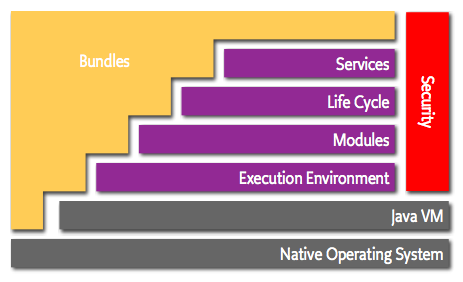
\includegraphics[width=0.7\linewidth]{Bilder/layering-osgi.png}
	\captionof{figure}[OSGi Architektur]{OSGi Architektur\footnotemark }
	\label{fig:osgi}
\end{minipage}
\footnotetext{Quelle: \url{http://www.osgi.org/Technology/WhatIsOSGi}}

\subsection{Tabellen}
In diesem Abschnitt wird eine Tabelle (siehe Tabelle \ref{tab:beispiel}) dargestellt.

\vspace{1em}
\begin{table}[!h]
	\centering
	\begin{tabular}{|l|l|l|}
		\hline
		\textbf{Name} & \textbf{Name} & \textbf{Name}\\
		\hline
		1 & 2 & 3\\
		\hline
		4 & 5 & 6\\
		\hline
		7 & 8 & 9\\
		\hline
	\end{tabular}
	\caption{Beispieltabelle}
	\label{tab:beispiel}
\end{table}

\pagebreak
\subsection{Auflistung}
Für Auflistungen wird die \textit{compactitem}-Umgebung genutzt, wodurch der Zeilenabstand zwischen den Punkten verringert wird.

\begin{compactitem}
	\item Nur
	\item ein
	\item Beispiel.
\end{compactitem}

\subsection{Listings}
Zuletzt ein Beispiel für ein Listing, in dem Quellcode eingebunden werden kann, siehe Listing \ref{lst:arduino}.

\vspace{1em}
\begin{lstlisting}[caption=Arduino Beispielprogramm, label=lst:arduino]
int ledPin = 13;
void setup() {
    pinMode(ledPin, OUTPUT);
}
void loop() {
    digitalWrite(ledPin, HIGH);
    delay(500);
    digitalWrite(ledPin, LOW);
    delay(500);
}
\end{lstlisting}

\subsection{Tipps}
Die Quellen befinden sich in der Datei \textit{bibo.bib}. Ein Buch- und eine Online-Quelle sind beispielhaft eingefügt. [Vgl. %\cite{buch}, \cite{online}]

Abkürzungen lassen sich natürlich auch nutzen (). Weiter oben im Latex-Code findet sich das Verzeichnis.
\pagebreak


\end{document}
